% This example poster is from Scientific Career Resources
%
% Author:
% Chris Rackauckas <contact@chrisrackauckas.com>
% http://www.chrisrackauckas.com
\RequirePackage{comfortaa}
\documentclass[paper=a0paper,papersize={48in,36in},landscape,dvipsnames]{umbcposter}
\renewcommand{\familydefault}{\sfdefault}

%%%%%%%%%%%%%%% GRAPHICS

\usepackage{graphicx}

\usepackage{pgfplots}
\usepackage{pgfplotstable}
\usepackage{tikz}
\usetikzlibrary{calc}
\usetikzlibrary{positioning,shapes,arrows, fit, shapes.geometric}

\pgfplotsset{compat=1.8}

\makeatletter
\pgfplotsset{
	/pgfplots/flexible xticklabels from table/.code n args={3}{%
		\pgfplotstableread[#3]{#1}\coordinate@table
		\pgfplotstablegetcolumn{#2}\of{\coordinate@table}\to\pgfplots@xticklabels
		\let\pgfplots@xticklabel=\pgfplots@user@ticklabel@list@x
	}
}
\makeatother

%%%%%%%% Misc


\begin{document}

\newcommand{\mytitle}{
    \tikz \node[
			text centered,
		    align=center,
            fill=white,
            draw=blue,                   % draw box border
            rounded corners=2ex,
            opacity=0.75,                % background opacity
            text opacity=.9,             % text opacity
            inner sep=0.1\headheight,  % padding around the text
        ] at (0,0) {
	        \Huge NovelPersepective:\\
	        \Huge Identifying Point of View Characters\\
	        {\huge Lyndon White, Roberto Togneri, Wei Liu, Mohammed Bennamoun}
    };    % don't forget the semicolon here!
}



\posterinit{
	%grid,
	background style = {left color = Apricot, right color = white},
	title = {\mytitle},
	right logo,       % use default
	left logo = {\includegraphics[height=.33\headheight]{UWA-Full-Hor-CMYK}},
	box/border style, % use default
	box/header style, % use default
	box/body style = {bottom color=blue!10, top color=red!5},
	box/all rounded,
}

\boxit{col = 0, at top, name=problem}{The Zebrafish Hindbrain}{

	\vspace{10pt}
}

\boxit{col = 0, below of = problem, name=box2}{The Interaction Network}{

	\vspace{5.3pt}
}

\boxit{at top, col = 1, name=box3}{The Proccess}{
	\resizebox{\textwidth}{!}{
		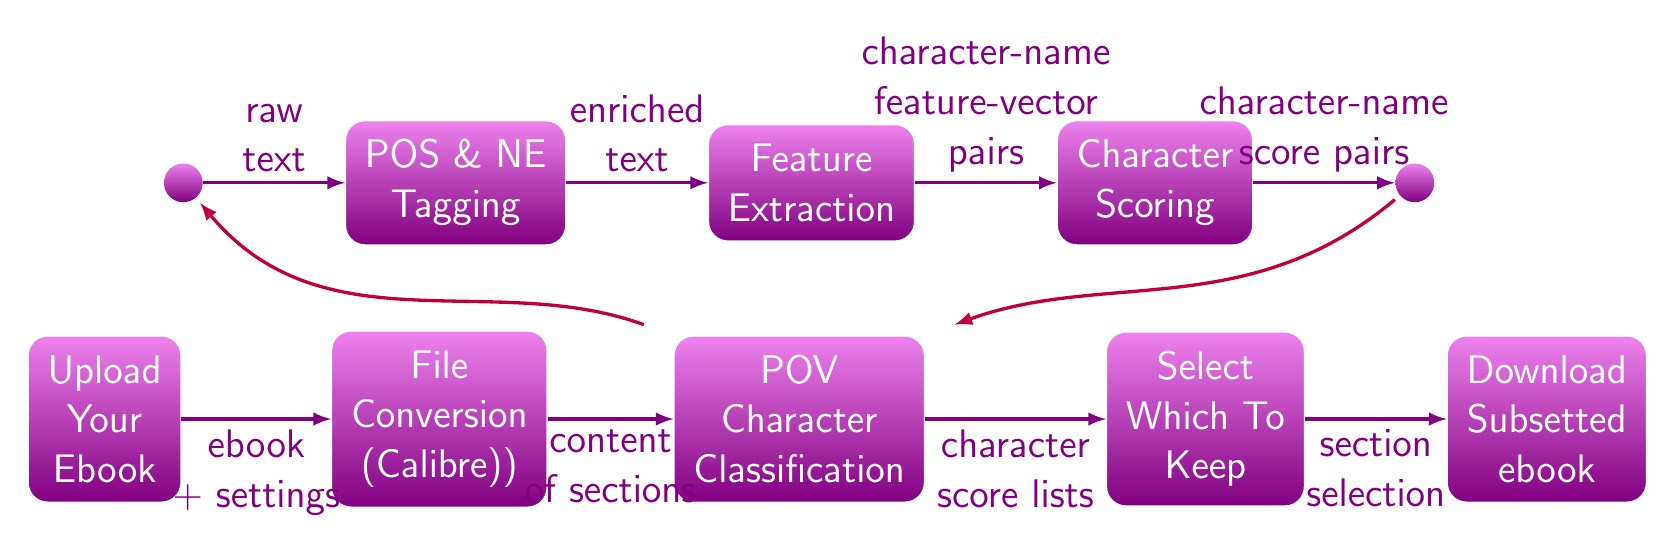
\begin{tikzpicture}[
		>=latex,
		every text node part/.append style={align=center},
		auto,
		node distance=1.8, 
		->,
		every edge/.append style={very thick, Purple, every node/.style={font=\Large}},
		every node/.append style={rounded corners=7pt, fancy, inner sep=7pt, font=\Large},
		gather/.style = { very thick, purple, shorten <= 0.4cm},
		fancy/.style= {draw=none, shade, 
			color=White,
			top color=Violet, bottom color=Purple
		}
		]	
		\begin{scope}[yshift=3cm]		
		\node(start1){};
		\node(enrich)[draw, right=of start1] {POS \& NE \\ Tagging};
		\node(features)[draw, right=of enrich] {Feature\\ Extraction};
		\node(scoring)[draw, right=of features] {Character\\Scoring};				
		\node(end)[right=of scoring] {};
		
		\path (start1) edge node[]{raw\\ text}  (enrich);
		\path (enrich) edge node[above]{enriched\\text} (features);
		\path (features) edge node[above]{character-name\\feature-vector\\pairs
		} (scoring);
		\path (scoring) edge node[above]{character-name\\score pairs
		} (end);
		\end{scope}
		
		\begin{scope}[xshift=-1cm]		
		\node(start)[draw] {Upload\\ Your \\Ebook};
		\node(convert)[draw, right=of start, xshift=0.1cm] {File\\Conversion\\(Calibre))};
		\node(classify)[draw, right=of convert, xshift=-0.2cm] {POV\\Character\\Classification};
		\node(select)[draw, right= of classify, xshift=0.5cm] {Select\\ Which To \\ Keep};
		\node(download)[draw, right=of select] {Download \\ Subsetted \\ ebook};
		
		\path (start) edge[below] node[below]{ebook \\ + settings}  (convert);
		\path (convert) edge[below] node[below]{content\\ of sections} (classify);
		\path (classify) edge[below] node[below]{character\\score lists} (select);
		\path (select) edge[below] node[below]{section\\selection} (download);	
		
		\draw[->, gather] (classify.north west) to[out=160, in=-50] (start1);
		\draw[<-, gather] (classify.north east) to[out=20, in=-140] (end);
		\end{scope}
		\end{tikzpicture}}
}

\boxit{below of = box3, col=1, name=box4}{The Fluctuation-Dissipation Theorem}{

}


\boxit{below of = box4, col = 1, name=solution}{Solution}{

}

\boxit{at top,col = 2, name=conclusions}{Conclusions}{

	\vspace{4pt}
}

\boxit{below of = conclusions,col = 2, name=future}{Future Directions}{

	\vspace{4pt}
}

\boxit{col=2, below of= future, name = refs}{Acknowledgments}{
	\vspace{3pt}
	\vspace{6.3pt}
}


\end{document}
